\documentclass[09pt,letterpaper]{article}
\usepackage[lmargin=2.4in,rmargin=0.5in,tmargin=1.0in,bmargin=1.0in]{geometry}\usepackage{notes}
\begin{document}


\begin{center}
\Large\textbf{1.5 – Applications of First-Order Differential Equations}\\
\normalsize (Sections 1.3.2, 1.3.3, 1.4.2)
\end{center}

%-------------------------------------------------------------
\section{Newton's Law of Cooling}

\subsection{Goal}
Newton's Law of Cooling describes how a hot object sitting in a cooler environment loses heat over time. Our goal is to learn how to model this law with differential equations. 


\subsection{Setup}
We want a model for 
\[
T(t) = \text{temperature of an object at time } t.
\]
We make the following assumptions:
\begin{itemize}
    \item The surrounding environment is held at a constant temperature $T_e$.
    \item The initial temperature of the object is $T_0$. 
    \item The object has a uniform temperature throughout (a.k.a. lumped thermal model).
    \item Heat is exchanged instantaneously and uniformly.
\end{itemize}

\subsection{Constant Cooling}
Imagine a freshly poured coffee, initially $T_0=200\degree $F, is placed in room temperature $T_e=70\degree $F. The goal is to find $T(t) = $ temperature of the coffee $t$ minutes later. Suppose the coffee cools by $5\degree $F per minute. Then a model for the coffee would be 
$$
    \frac{dT}{dt} = -5, \quad T(0)=200.
$$
Notice that $T'<0$ which indicates cooling. The solution is $T(t)=200-5t$. There is an issue with this model. This solution says after 26 minutes, the coffee reaches room temperature. Then it gets colder and colder. The coffee reaches freezing temperature after 40 minutes. There are two reasons why this model is not realistic:
\begin{enumerate}
    \item the coffee shouldn't continue to get colder after reaching $70\degree $F.
    \item the environment temperature should affect the rate of cooling.
\end{enumerate}


\subsection{Newton’s Law of Cooling}

\textbf{Newton’s Law of Cooling} states:

\begin{quote}
\textit{The rate of change of the temperature of an object is proportional to the difference between the temperature of the object and that of the surrounding environment.}
\end{quote}
Mathematically, this gives the differential equation
\[
\boxed{
\frac{dT}{dt} = -h\,(T - T_e),
}
\]
where $h>0$ is the \textbf{heat transfer coefficient}. Let's examine each component of this model:
\[
\underbrace{\frac{dT}{dt}}_{
  \begin{array}{c}
    \text{rate of change }\\
    \text{of the}\\
    \text{object's temperature}
  \end{array}
}
=
\underbrace{-h}_{
  \begin{array}{c}
    \text{negative}\\
    \text{proportionality}\\
    \text{constant}
  \end{array}
}
\,\underbrace{(T-T_e)}_{
  \begin{array}{c}
    \text{temperature diff.}\\
    \text{between the}\\
    \text{object and room}
  \end{array}
}.
\]
To understand this model, let's consider three different levels of temperature:
\begin{enumerate}
    \item The object is much hotter than the environment $T\gg T_e$. 
        $$T\gg T_e \implies T'\ll 0\implies \text{fast cooling}$$
    \item The object is warmer than the environment $T > T_e$
        $$ T >T_e \implies T'<0 \implies \text{regular cooling}$$
    \item The object cools down to the environment temperature $T=T_e$
    $$ T = T_e \implies T'=0\implies \text{fixed temperature}$$
\end{enumerate}
This model addresses the unrealistic features of the constant cooling model. The cooling is affected dynamically by the environment, and the object never gets cooler than the environment.

\begin{example}[1]{    
You pour a freshly brewed cup of coffee at $200^\circ$F.
The coffee cools down with a heat coefficient of $h=0.08$ per minute as you sip on the coffee in room temperature  70\degree F. You do not want the coffee to reach 120\degree F, at which point the flavors become muted and flat. How long do you have to drink the coffee? 
}

\paragraph{Step 1: Set up the model.} We let $T(t)$ be the temperature of the coffee after $t$ minutes. Let $T_e=70\degree$F be the room temperature. By Newton’s law of cooling, the temperature $T(t)$ satisfies
\[
\begin{aligned}
\frac{dT}{dt} &= -h\bigl(T - T_e\bigr)\\
\frac{dT}{dt} &= -0.08\bigl(T - 70\bigr)
\end{aligned}
\]
with the initial condition $T(0)=200\degree$F. 
\paragraph{Step 2: Solve the model.} The DE can be solved with integrating factors or by separation. Let's do separation:
\begin{align*}
\frac{dT}{dt} &= -0.08\bigl(T - 70\bigr)\\
\frac{dT}{T - 70} &= -0.08\,dt\\    
\int \frac{dT}{T - 70} &= \int -0.08\,dt\\
\ln|T - 70| &= -0.08t + C\\
T-70 &= Ce^{-0.08t}\\
T(t)&= Ce^{-0.08t}+70
\end{align*}
The initial temperature is $T(0)=200$, so
\[
T(0) =  C +70 \equiv 200\quad \Rightarrow \quad C = 130.
\]
Thus the temperature of the coffee is 
\[
\boxed{
T(t) = 70 + 130e^{-0.08t}.
}
\]
\paragraph{Step 3: Use the solution.}
We now solve for the time when $T(t)=120$:
\begin{align*}
120 &= 70 + 130e^{-0.08t} \\
50 &= 130e^{-0.08t} \\
\frac{50}{130} &= e^{-0.08t} \\
\ln\!\left(\frac{50}{130}\right) &= -0.08t \\
t &= -\frac{1}{0.08}\ln\!\left(\frac{50}{130}\right) \approx 11.94.
\end{align*}
You have about 12 minutes to finish your coffee before it reaches $120\degree$.
\end{example}

% \paragraph{Remark:} The solution to the model is an exponential decay $T(t) = 70 + 130e^{-0.08t}$. The solution curve $T(t)$ starts at $T_0=200$ and decays down to the room temperature $T_e=70$. There is a horizontal asymptote at $T=T_e$. The temperature of the coffee will never fall below $70\degree$F.

%-------------------------------------------------------------
% \subsection{General Heat Transfer}

% Heat naturally flows from regions of higher temperature to regions of lower temperature.
% Newton’s Law of Cooling describes how this transfer occurs between an object and its surrounding environment.
% When an object is hotter than its environment, heat flows outward and the object cools.
% When an object is colder than its environment, heat flows inward and the object warms.

% Both processes are described by the \emph{same mathematical model}.
% The direction of heat flow is determined entirely by the sign of the temperature difference.

\subsection{Heating versus Cooling}

Newton's law of cooling assumes the initial temperature $T_0$ is hotter than the environment. But what if the object is \textit{colder} than the environment? We would expect the object to dynamically warm up to environment temperature. It turns out that the model for heating is \textit{exactly the same} as the model for cooling
\[
T' = -h(T - T_e),
\]
where $h>0$. For example, if you stick a room-temperature turkey into a 400 $\degree$F oven, then the model for the turkey is 
$$
T' = -h(T-400), \quad T(0)=70.
$$
Since the temperature of the turkey $T$ is always under $400\degree$F, the quantity $T-400$ must be negative. Therefore, the derivative is always positive
$$
T'=-h(T-400) > 0
$$
which indicates that the cold turkey is heating up. The table below illustrates how the sign of $T'$ appropriately changes according to the situation (heating vs. cooling).

\begin{center}
\renewcommand{\arraystretch}{1.4}
\begin{tabular}{|c|c|c|}
\hline
\textbf{Situation} & \textbf{Sign Analysis} & \textbf{Behavior} \\
\hline
Object warmer than environment 
& 
$T-T_e>0 \;\Rightarrow\; T'<0$ 
& 
Object cools down toward $T_e$ \\
\hline
Object colder than environment 
& 
$T-T_e<0 \;\Rightarrow\; T'>0$ 
& 
Object heats up toward $T_e$ \\
\hline
Object and environment same temp 
& 
$T-T_e=0 \;\Rightarrow\; T'=0$ 
& 
Object's temp is fixed \\
\hline
\end{tabular}
\end{center}

\subsection{Steady State Temperature}

Whether the object is cooling or heating the solution to the initial value problem 
$$
\begin{dcases}
    T' = -h(T-T_e) \\
    T(0)=T_0
\end{dcases}
$$
is the function 
\[
T(t) = T_e + (T_0 - T_e)e^{-ht},
\]
where $T_0=T(0)$ is the initial temperature of the object. When plotted on a graph, the solution curve is an exponential decay with a vertical shift. The solution appears slightly different depending on whether the object is heating or cooling. See the figure below. 
\begin{figure}[H]
    \centering
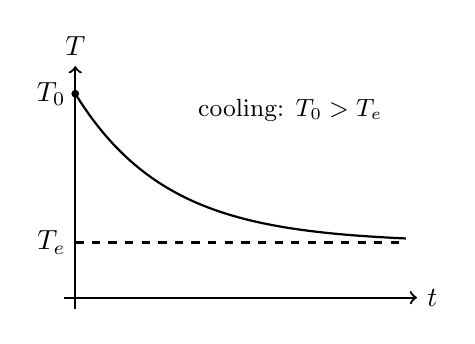
\begin{tikzpicture}[scale=0.7]
    % Axes
    \draw[->,thick] (-0.2,0) -- (6.2,0) node[right] {$t$};
    \draw[->,thick] (0,-0.2) -- (0,4.2) node[above] {$T$};

    % Te line
    \draw[dashed,thick] (0,1.0) -- (6,1.0);
    \node[left] at (0,1.0) {$T_e$};

    % Cooling curve: T(t) = Te + (T0-Te)e^{-kt}
    \draw[thick,domain=0:6,samples=120]
        plot (\x,{1.0 + 2.7*exp(-0.6*\x)});

    % Initial temperature marker
    \fill (0,3.7) circle (2pt);
    \node[left] at (0,3.7) {$T_0$};

    % Label
    \node at (3.9,3.4) {\small cooling: $T_0>T_e$};

\end{tikzpicture}
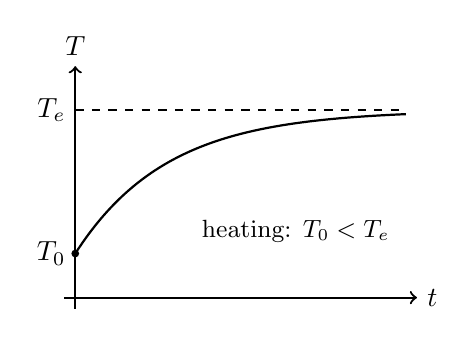
\begin{tikzpicture}[scale=0.7]
    % Axes
    \draw[->,thick] (-0.2,0) -- (6.2,0) node[right] {$t$};
    \draw[->,thick] (0,-0.2) -- (0,4.2) node[above] {$T$};

    % Te line
    \draw[dashed,thick] (0,3.4) -- (6,3.4);
    \node[left] at (0,3.4) {$T_e$};

    % Heating curve: T(t) = Te + (T0-Te)e^{-kt} with T0<Te
    \draw[thick,domain=0:6,samples=120]
        plot (\x,{3.4 - 2.6*exp(-0.6*\x)});

    % Initial temperature marker
    \fill (0,0.8) circle (2pt);
    \node[left] at (0,0.8) {$T_0$};
    % Label
    \node at (4.0,1.2) {\small heating: $T_0<T_e$};
\end{tikzpicture}
    \caption{The solution to the heat transfer model is always an exponential decay. The left shows the an object cooling down to $T_e$. The right shows the }
\end{figure}
The parameter $T_e$ represents the temperature of the environment, but it is also the final temperature of the object. For instance, if a hot cup of coffee is sitting in room temperature for a long time, then the coffee will eventually reach room temperature. For this reason, we call $T_e$ the \textbf{steady state} temperature. It is \textit{steady} in the sense that the object's temperature stops changing after it reaches $T_e$. 

\subsection{Variable Environment Temperature}
Lastly, let us consider a non-static environmental temperature. Suppose you wanted to model $T(t)=$ the temperature of a pond after $t$ days. The model
$$
    T'=-h(T-T_e)
$$
isn't appropriate since the temperature $T_e$ would not remain constant over the span of a month. To make this model more realistic, we write
\[
\frac{dT}{dt}=-h\bigl(T-Q(t)\bigr),
\]
where $Q(t)$ is the temperature of the environment surrounding the pond. For example, the weather outside varies like a sine wave over 24 hours. Separation of variables cannot be used to solve this equation. However, notice that we can write the model as 
$$
\frac{dT}{dt} + hT=h\,Q(t),
$$
which is the normal form. This can be solved using integrating factors.

%-------------------------------------------------------------
\section{Law of Conservation}

\subsection{Store Example}
Suppose you work as an analyst at a grocery store. Your boss tasks you with calculating the rate at which customers are entering/leaving the store. You let $x(t)=$ the number of customers at time $t$. Therefore, you must calculate the derivative $x'$.

\subsection{Calculating $x'$}
The quantity $x'$ represents the rate at which customers are entering/leaving the store. One way to calculate $x'$ it by counting the number of customers in the store, waiting $\Delta t$ minutes, and then recounting the number of customers again. Then you have the approximation
$$
x' \approx \frac{x_{\text{after}}-x_{\text{before}} }{\Delta t}.
$$
There is nothing mathematically incorrect about this approximation, but physically counting every customer in the store can be difficult or lead to inaccuracies. 

\subsection{Net Flux}
There is a more clever way to approximate $x'$. You can stand by the entrance of the store and then count the number of customers that come in and out over a time interval $\Delta t$. Then you have the approximation 
$$
x' \approx   x_{in} -x_{out},
$$
where $x_{in}$ and $x_{out}$ have units number of customers per $\Delta t$. This is simpler to count physically and is less error prone. The difference between the rate in and the rate out is called the \textbf{net flux}. 

\subsection{Law of Conservation}
Scientists figured out long ago that calculating the rate of change of some material in a region can be done by observing the flux around the \textit{boundary} rather than measuring quantities of the \textit{interior}. Put simply, the law of conservation says
$$
\frac{d}{dt}(\text{quantity in a region}) = \text{rate in} - \text{rate out}. 
$$
This may seem like common sense. This is a very powerful concept that is used extensively to derive physical laws. 

%-------------------------------------------------------------

\section{Chemostat Model}

In this section, we discuss the \textit{mixing problem} or the \textit{chemostat model}. The model is derived from the conservation of mass.

\subsection{What is a Chemostat?}

The \textbf{chemostat} is a mixing tank with a constant stream of fluid coming in and out of it. The incoming fluid contains some material that is then mixed into the tank. We are concerned about the concentration of the material in the tank. Here are some examples: 
\begin{itemize}
    \item a biological growth chamber,
    \item amount of pollution in a lake,
    \item amount of air pollution in a room with ventilation, 
    \item amount of some chemical in an organ.
\end{itemize}
Generally, we are interested in any scenario in which a contaminated fluid enters a chamber, mixes with the fluid in the chamber, and the fluid leaves the chamber at the same rate.

\subsection{Setup}

\paragraph{Assumptions}
\begin{itemize}
    \item There is a mixing tank with a fixed volume of fluid.
    \item The mixing tank receives fluid from a source tank with a fixed concentration.
    \item Fluid flows into and out of the tank at the \underline{same rate}.
    \item Incoming fluid mixes \underline{instantly} with the fluid in the tank.
\end{itemize}

\paragraph{Quantities and SI Units}
The goal is to determine 
$$C(t)  \;(\text{units }kg/m^3)$$
which represents the concentration of the substance in the mixing tank at time $t$. These are the other fixed parameters
\begin{itemize}
    \item $V$ ($m^3$) = volume of fluid in the tank.
    \item $q$ ($m^3/s$) = speed of fluid coming in and out of the tank.
    \item $C_{\text{in}}$ ($kg/m^3$)  = concentration of material in the fluid flowing in.
    \item $C_{0}$ ($kg/m^3$)  = initial concentration of material in the tank.
\end{itemize}

\begin{figure}[H]
    \centering
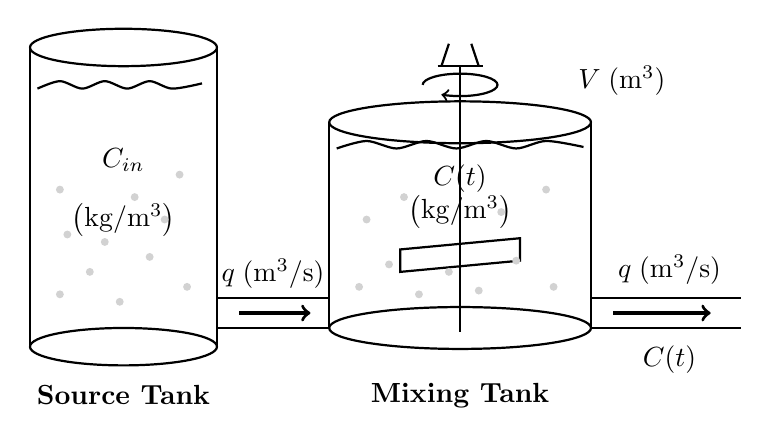
\begin{tikzpicture}[scale=0.95]
% -------------------------------------------------
% Source reservoir
% -------------------------------------------------
\draw[thick] (-5,0) -- (-5,4);
\draw[thick] (-2.5,0) -- (-2.5,4);

% Top and bottom ellipses
\draw[thick] (-5,4) arc[start angle=180,end angle=360,
    x radius=1.25,y radius=0.25];
\draw[thick] (-2.5,4) arc[start angle=0,end angle=180,
    x radius=1.25,y radius=0.25];

\draw[thick] (-5,0) arc[start angle=180,end angle=360,
    x radius=1.25,y radius=0.25];
\draw[thick] (-2.5,0) arc[start angle=0,end angle=180,
    x radius=1.25,y radius=0.25];

% Liquid surface
\draw[thick]
    plot[smooth] coordinates {
    (-4.9,3.45) (-4.6,3.55) (-4.3,3.45)
    (-4.0,3.55) (-3.7,3.45) (-3.4,3.55)
    (-3.1,3.45) (-2.7,3.52)
    };

% Source label
\node at (-3.75,2.5) {$C_{\text{in}}$};
\node[align=center] at (-3.75,1.7)
    {$\left(\mathrm{kg/m^3}\right)$};

% Solute particles
\foreach \x/\y in {
    -4.6/0.7,-4.2/1.0,-3.8/0.6,-3.4/1.2,
    -2.9/0.8,-4.5/1.5,-4.0/1.4,-3.2/1.7,
    -4.6/2.1,-3.6/2.0,-3.0/2.3
}{
   \fill[gray!35] (\x,\y) circle (1.5pt);
}

% -------------------------------------------------
% Inflow pipe
% -------------------------------------------------
\draw[thick] (-2.5,0.65) -- (-1.0,0.65);
\draw[thick] (-2.5,0.25) -- (-1.0,0.25);

\draw[->,very thick] (-2.2,0.45) -- (-1.25,0.45);
\node[above] at (-1.75,0.65)
    {$q\;(\mathrm{m^3/s})$};

% -------------------------------------------------
% Mixing tank
% -------------------------------------------------
\draw[thick] (-1,0.25) -- (-1,3);
\draw[thick] (2.5,0.25) -- (2.5,3);

% Tank top
\draw[thick] (-1,3) arc[start angle=180,end angle=360,
    x radius=1.75,y radius=0.28];
\draw[thick] (2.5,3) arc[start angle=0,end angle=180,
    x radius=1.75,y radius=0.28];

% Tank bottom
\draw[thick] (-1,0.25) arc[start angle=180,end angle=360,
    x radius=1.75,y radius=0.28];
\draw[thick] (2.5,0.25) arc[start angle=0,end angle=180,
    x radius=1.75,y radius=0.28];

% Liquid surface
\draw[thick]
    plot[smooth] coordinates {
    (-0.9,2.65) (-0.5,2.75) (-0.1,2.65)
    (0.3,2.75) (0.7,2.65) (1.1,2.75)
    (1.5,2.65) (1.9,2.75) (2.4,2.67)
    };

% -------------------------------------------------
% Mixer
% -------------------------------------------------
\draw[thick] (0.75,3.75) -- (0.75,0.2);

% Motor / handle
\draw[thick] (0.45,3.75) -- (1.05,3.75);
\draw[thick] (0.5,3.75) -- (0.6,4.05);
\draw[thick] (1.0,3.75) -- (0.9,4.05);

% % Impeller blades
\draw[thick]
    (-0.05,1.00) --
    (-0.05,1.30) --
    (1.55,1.45) --
    (1.55,1.15) --
    cycle;

% Rotation arrow
\draw[->,thick]
    (0.25,3.5) arc[start angle=180,end angle=-120,
    x radius=0.5,y radius=0.15];

% -------------------------------------------------
% Tank labels
% -------------------------------------------------
\node at (0.75,2.25) {$C(t)$};
\node[align=center] at (0.75,1.8)
    {$\left(\mathrm{kg/m^3}\right)$};

\node[right] at (2.2,3.55)
    {$V\;(\mathrm{m^3})$};

% Solute particles in tank
\foreach \x/\y in {
    -0.6/0.8,-0.2/1.1,0.2/0.7,0.6/1.0,
    1.0/0.75,1.5/1.15,2.0/0.8,
    -0.5/1.7,0.0/2.0,1.3/1.8,1.9/2.1
}{
     \fill[gray!35] (\x,\y) circle (1.5pt);
}

% -------------------------------------------------
% Outflow pipe
% -------------------------------------------------
\draw[thick] (2.5,0.65) -- (4.5,0.65);
\draw[thick] (2.5,0.25) -- (4.5,0.25);

\draw[->,very thick] (2.8,0.45) -- (4.1,0.45);

\node[above] at (3.55,0.7)
    {$q\;(\mathrm{m^3/s})$};

\node[below] at (3.55,0.15)
    {$C(t)$};

% Tank labels
\node[font=\bfseries] at (-3.75,-0.65) {Source Tank};
\node[font=\bfseries] at (0.75,-0.65) {Mixing Tank};
% -------------------------------------------------
% Temporary positioning grid
% -------------------------------------------------
% \draw[step=0.5,gray!30,very thin]
%     (-5.5,-0.5) grid (5,4.5);
% \draw[step=1,gray!60,thin]
%     (-5.5,-0.5) grid (5,4.5);
% \foreach \x in {-5,-4,...,5}
%     \node[below,font=\scriptsize] at (\x,-0.5) {\x};
% \foreach \y in {0,1,...,4}
%     \node[left,font=\scriptsize] at (-5.5,\y) {\y};

\end{tikzpicture}

\caption{Chemostat model. Fluid with concentration $C_{\text{in}}$
enters the tank at volumetric flow rate $q$. The tank has constant
volume $V$ and concentration $C(t)$. Perfect mixing implies that the
outgoing fluid also has concentration $C(t)$.}
\end{figure}

%-------------------------------------------------------------
\subsection{The Model}

We will derive the differential equation for $C(t)$ using the Law of Conservation. The total amount of salt \emph{inside} the mixing tank at time $t$ is
\[
\text{mass} \;(m) = \text{volume} \;(m^3) \times \text{concentration} \;(kg/m^3)= V\,C(t).
\]
Water enters the tank at a speed $q$ with a salt concentration $C_{\text{in}}$, so the rate in is
\[
\text{rate in} \;(kg/s) = \text{fluid velocity}\;(m^3/s)\times \text{concentration}\;(kg/m^3)  = q\;\,C_{\text{in}}.
\]
Water leaves the tank at speed $q$ with concentration $C(t)$, so
$\text{rate out} = q\,C(t).$
Applying conservation of mass,
\begin{align*}    
\frac{d}{dt}(\text{quantity in a region}) &= \text{rate in} - \text{rate out}\\
\frac{d}{dt}\bigl(\underbrace{{V\,C(t)}\bigr)}_{\text{rate of change of salt}} &= \underbrace{q\,C_{\text{in}}}_{\text{rate in}} - \underbrace{q\,C(t)}_{\text{rate out}}.
\end{align*}

Since volume $V$ is constant, this simplifies to
\[
V\,\frac{dC}{dt} = q\bigl(C_{\text{in}} - C\bigr).
\]
Dividing both sides by $V$ gives the chemostat model:
\[
\boxed{
\frac{dC}{dt} = \frac{q}{V}\bigl(C_{\text{in}} - C\bigr).
}
\]
We can use this DE as the model for the brine-mixing problem.

\subsection{Word Problem}
A soup factory has a large supply of salted water, or brine, that is too salty to use in its product. To dilute the brine, the factory pumps it into a $1000$ L mixing tank that initially contains only pure water and is kept perfectly mixed at all times. The brine enters the tank at a rate of $20$ L/min with a salt concentration of $80$ g/L, while the well-mixed solution leaves the tank at the same rate of $20$ L/min so that the total volume remains constant. The factory wants to stop the process when the concentration of salt in the tank reaches $10$ g/L, which is the ideal salinity for its soup. How long, in minutes, will it take for the solution in the tank to reach this concentration?
%-------------------------------------------------------------
\begin{example}[2]{

A factory pumps brine into a mixing tank that initially contains pure water. The tank is perfectly mixed and kept at constant volume by pumping out at the same rate.

\begin{itemize}
    \item Tank volume: $V=1000$ L.
    \item Flow rate in/out: $q=20$ L/min.
    \item Inflow concentration: $C_{\text{in}}=80$ g/L.
    \item Initial condition: $C(0)=0$ (pure water).
\end{itemize}
\textbf{Goal:} Find the time (minutes) when $C(t)=10$ g/L.
}


\paragraph{Step 1: Set up the model.}
\[
C'=\frac{20}{1000}(80-C)=\frac{1}{50}(80-C)
=1.6-\frac{1}{50}C,
\qquad
C(0)=0.
\]
Rewrite in linear form:
\[
C' + \frac{1}{50}C = 1.6.
\]

\paragraph{Step 2: Solve the model.}
Using the integrating factor $\mu(t)=e^{t/50}$,
\[
\frac{d}{dt}\left(e^{t/50}C\right)=1.6e^{t/50}.
\]
Integrate:
\[
e^{t/50}C = 1.6\int e^{t/50}\,dt + K
=1.6(50)e^{t/50}+K
=80e^{t/50}+K.
\]
So
\[
C(t)=80+Ke^{-t/50}.
\]
Apply $C(0)=0$:
\[
0=80+K \Rightarrow K=-80.
\]
Thus
\[
\boxed{
C(t)=80\left(1-e^{-t/50}\right)\ \text{g/L}.
}
\]

\paragraph{Step 3: Use the solution.}
Set $C(t)=10$:
\begin{align*}
10 &= 80\left(1-e^{-t/50}\right)\\
\frac{1}{8} &= 1-e^{-t/50}\\
e^{-t/50} &= \frac{7}{8}\\
t &= -50\ln\left(\frac{7}{8}\right)\approx 6.68.
\end{align*}
\[
\boxed{t \approx 6.68\ \text{minutes}.}
\]
\end{example}

%-------------------------------------------------------------
\section{Draining Chemostat}
In previous mixing problems, we assumed that fluid enters and leaves the tank at the same rate, so the volume stays constant. What if we can control the incoming flow rate and the outgoing flow rate? This will slightly complicate the model but it is still solvable.

\subsection*{The New Setup}
Consider the chemostat model for the concentration of material in the tank at time $t$. This time we assume that the speed of the fluid coming into the tank is slower than the speed of the fluid going out of the tank. We again assume that the incoming fluid mixes instantly with the fluid in the tank. We will assume that the tank has some initial volume of fluid. Here are the parameters:
\paragraph{Variables and SI Units}
\begin{itemize}
    \item $V(t)$ ($m^3$) = volume of fluid in the tank.
    \item $V_0$  $(m^3)$ = initial volume of fluid. 
    \item $q_{\text{in}}$ ($m^3/s$) = speed of fluid coming into the tank.
    \item $q_{\text{out}}$ ($m^3/s$) = speed of fluid going out of the tank.
    \item $C_{\text{in}}$ ($kg/m^3$)  = concentration of material in the fluid flowing in.
    \item $C_{0}$ ($kg/m^3$)  = initial concentration of material in the tank.
\end{itemize}
We must have $q_{\text{out}} > q_{\text{in}}$.

\subsection*{Fluid in the Tank}
Since inflow and outflow rates may differ, the rate of change of the volume of the fluid is 
$$
\frac{dV}{dt} = q_{\text{in}} - q_{\text{out}}.
$$
This is a simple DE because the RHS is a constant. We also have the initial condition $V(0)= V_0$. Solving this DE gives us the formula for volume
\[
V(t) = (q_{\text{in}} - q_{\text{out}})t +K.
\]
We may use the initial condition $V(0)=V_0$ to solve for $K$. We get $K=V_0$ which yields the formula for the volume of fluid in the tank:
\[
V(t) = (q_{\text{in}} - q_{\text{out}})t +V_0.
\]
When the tank is fully drained, the model is no longer relevant. We only care about the time range from $0<t<t_{fin}$. We can use this to determine when the become becomes empty by setting $V(t_{fin})=0$ and solving for $t_{fin}$. 

\subsection*{The New Model}
In the original model with equal flow rates, the conservation law gave us the equation $(VC)' = qC_{in} - qC$. In our new model with variable volume $V(t)$ and differing flow rates, the equation is 
$$
(V(t)\, C(t))' = q_{\text{in}} \,C_{\text{in}} - q_{\text{out}} \,C.
$$
For this model, you must use product rule for derivatives to simplify the LHS. I leave it as an exercise for you to show that the new model can be written in the normal form:
\[
C'(t)
+
\left(
 \frac{q_{\text{out}}+V'(t)}{V(t)}
\right) C(t)
=
\frac{q_{\text{in}}}{V(t)}\,C_{\text{in}}.
\]
The draining chemostat model is slightly more complicated but it is still a linear first-order DE. You can solve this using the method of integrating factors.

\end{document}
